\documentclass[a4paper, 12pt]{report}

\usepackage{geometry}
\usepackage{graphicx}
\usepackage{amsmath, amsfonts, amssymb, amsthm}
\usepackage{lmodern}
\usepackage[colorlinks=true,
			citecolor=blue,
			linkcolor=blue,
			]{hyperref}
\usepackage{enumerate}
\usepackage{enumitem}
\usepackage{comment}
\usepackage{float}
\usepackage{a4wide}
\usepackage{setspace}
\usepackage [
	n, % or lambda advantage , 
	operators , 
	sets,
	adversary , 
	landau , 
	probability , 
	notions ,
	logic ,
	ff, 
	mm,
	primitives ,
	events , 
	complexity , 
	%oracles , 
	asymptotics , 
	keys,
	advantage
]{cryptocode}
\usepackage{tabularx}
\usepackage{forest}
\usepackage[bottom]{footmisc}
\usepackage{enumitem}
\usepackage[normalem]{ulem}
\useunder{\uline}{\ul}{}
% TODO add code (package minted)
% \usepackage{minted}


\begin{document}

\newcommand\Title{Privacy-Preserving Contact Discovery with Applications to End-to-End Encrypted Messaging and Mobile-First Cryptocurrencies}
\newcommand\Author{Nicolas Mohnblatt}
\newcommand\Supervisor{Dr. Philipp Jovanovic}
\newcommand\Degree{MSc in Information Security}


% ENVIRONMENTS
\newtheorem{definition}{Definition}[chapter]
\newtheorem{theorem}{Theorem}[chapter]
\newtheorem{secgame}{Attack Game}[chapter]


% SHORTHAND NOTATIONS
	% Groups
	\newcommand{\Gzero}{\ensuremath{\mathbb{G}_0}}
	\newcommand{\Gone}{\ensuremath{\mathbb{G}_1}}
	\newcommand{\Gt}{\ensuremath{\mathbb{G}_T}}

	% Crypto
	\newcommand{\Keygen}{\ensuremath{\mathsf{KeyGen}}}
	\newcommand{\Sign}{\ensuremath{\mathsf{Sign}}}
	\newcommand{\Verif}{\ensuremath{\mathsf{Verify}}}
	\newcommand{\msk}{\mathbf{msk}}
	\newcommand{\mpk}{\mathbf{mpk}}
	\newcommand{\Exp}[1]{\mathrm{EXP}({#1})}


	% Maths
	\newcommand{\Pair}[2]{e\left(#1, #2 \right)} % Pairing operation
	
	% L-R PRFs
	\newcommand{\keyleft}[1]{k_{#1,\mathrm{LEFT}}}
	\newcommand{\keyright}[1]{k_{#1,\mathrm{RIGHT}}}

	% Variables
	\newcommand{\id}{\mathtt{id}}
	\newcommand{\acc}{\mathbf{acc}}
	\newcommand{\addr}{\mathbf{addr}}
	\newcommand{\contacts}[1]{\mathcal{C}_{#1}}

\onehalfspacing
\newcommand{\maketitleucl}{
    \newpage%
    \null%
    \vspace*{5em}%

    \begin{center}%
        {\huge  \Title}\\[5em]%
        {\Large \bfseries \Author\footnote{\textbf{Disclaimer:} this report is substantially the result of my own work except where explicitly indicated in the text. The report may be freely copied and distributed provided the source is explicitly acknowledged.}}\\[2em]%
        {\large  \bfseries Supervised by \Supervisor}\\
    \end{center}%
    \vfill%
    \begin{center}%
   
    \vspace{2em}
    
    A dissertation submitted in partial fulfilment \\
    of the requirements for the degree of \\
    \textbf{\Degree} \\
    at \\
    \textbf{University College London}.
    \end{center}%
    
    
    \vspace{2em}%
    
    
%    \begin{center}%
%    Department of Computing \\
%    University College London\\
%    \end{center}%
%    \vspace{2em}%
    \begin{center}%
    \today%
    \end{center}%
    \vspace{4em}%
    
  

\thispagestyle{empty}



%      
%\clearpage%
%I, \Author , confirm that the work presented in this thesis is my own.
%Where information has been derived from other sources, I confirm that this has been indicated in the work.
%\thispagestyle{empty}
%\clearpage%

}

\maketitleucl

% IMPORT SECTIONS


\begin{abstract}
	\paragraph{} In this report we consider means to perform privacy-preserving contact discovery on mobile devices. Contact discovery is a crucial initial step for any social application. Current methods reveal private information or require users to reason about cryptography. We introduce an approach based on non-interactive identity-based key exchange protocols (NI-IBKE). Our scheme provides users with cryptographic material which is entirely managed by a client-side application. Users can input their contacts' phone numbers (or an equivalent human-readable identifier) to compute shared secret keys on-device. Our system relies on a $t$-out-of-$n$ trust assumption with respect to a decentralised service. We show that the desired privacy property holds in the random oracle model under the decisional bilinear Diffie-Hellman assumption. We provide estimates of the system's performance in the wild. These show that our scheme is applicable but will require optimisations or a long bootstrapping period if used for applications with billions of users. Finally we describe a simple proof-of-concept implementation as well as applications of the scheme for end-to-end messaging or mobile-first cryptocurrencies.

\end{abstract}

\newpage

\renewcommand\abstractname{Acknowledgements}
\begin{abstract}
	
\end{abstract}
\hypersetup{linkcolor=black} % Change link colour for TOC
\setcounter{tocdepth}{1}
%{\singlespacing \tableofcontents} % TOC in single spacing
\tableofcontents
\hypersetup{linkcolor=blue} % Change back link colour


\chapter{Introduction}
\label{chap:intro}


\paragraph{} Privacy-oriented services such as end-to-end encrypted messaging are increasingly popular \cite{e2epopular}. While they provide strong cryptographic guarantees for the confidentiality of message contents, many still leak or gather user-related data. This is particularly the case during a setup stage known as \textit{contact discovery}. As a result, some of these applications gain access to their users' address books and therefore their mobile social graph \cite{Telegram,WhatsApp}. In this project, we are interested in performing \textit{contact discovery} in a privacy-preserving manner while remaining practical for mobile applications with billions of users.

\section{What is contact discovery?}

\paragraph{} \textit{Contact discovery} (alternatively \textit{contact matching}) simply refers to the process by which users of a service are able to find people they know on the said service. The applied method is largely determined by the amount of information users choose to make public. In the case of networks such as Facebook or LinkedIn, users are encouraged to register with --- and publish --- their legal names and can therefore be found through a simple search. In the cases we study, users are registered using pre-existing human-readable identifiers such as their phone numbers or email addresses. This information is kept private by the service such that only users with prior knowledge of each other's identifier can communicate.

\paragraph{} As a user signs up to such a service, she will already hold an \textit{address book} -- a register that links people (often referred to as \textit{contacts}) to their identifier. However, phone numbers and email addresses are identifiers generated by other services and there is no guarantee that all her \textit{contacts} are using the new service. Thus in this context, \textit{contact discovery} is more precisely defined as the process by which a user can discover whether or not her \textit{contacts} are using a specific service. Notice that such a process is not only a necessary initialisation step; it must also be regularly refreshed to ensure users keep an up-to-date view of the contacts they can address.


\section{The privacy challenge}

\paragraph{} The simplest way to perform contact discovery is arguably to send one's address book to the service operator, allowing them to compute the intersection between the address book and the list of registered users. This is in fact how the popular messaging services WhatsApp and Telegram perform their contact matching \cite{Telegram,WhatsApp}. Although efficient, this approach reveals large amounts of private information about  users and their contacts, including those that are not register for the service. The service operator is able to construct a social graph of its users and their first connections, allowing it to check for individual connections at will or under government pressure. Such information may discourage whistleblowers from ever speaking up, in fear that their identity may be revealed if they are linked to journalists.


\paragraph{Naive hashing --}A naive approach using only cryptographic hash functions will also fail to meet our goal \cite{Kales19, Signal:Difficulty}. Alice could upload hashes of her contacts' identifiers for the service operator to compare against hashes of the registered users' identifiers. While this approach is efficient and yields the desired result, it will still leak Alice's address book.

Indeed, although the cryptographic hash function is pre-image resistant, the set of possible pre-images is small enough that hashes can be precomputed into a dictionary and used to find the identifiers that underly the uploaded hashes \cite{Signal:Difficulty}. Salting these hashes to avoid offline computations renders the system unusable since the service operator would be required to hash the set of registered identifiers using a different salt for each attempt at contact discovery \cite{Kales19}.

\paragraph{Advanced approaches and Efficiency --} In light of the above, more advanced approaches have been developed to perform privacy-preserving contact discovery. We cover these in greater detail in \autoref{chap:litreview}. The issue with such approaches is that they introduce additional complexity through computations, communication requirements, storage requirements or a combination thereof.

In the context of the services we study, contact discovery needs to be performed on mobile devices on a regular basis. These devices are less powerful than modern desktop computers and rely on rechargeable batteries. A computation-intensive process ran regularly on such a device could quickly drain its battery. Furthermore we must allow the process to scale elegantly with the number of registered users, and assume that it can grow to the order of billions.

Efficiency therefore constitutes a priority in the design of such contact discovery schemes. It will also provide a benchmark to evaluate systems against each other, provided that they guarantee a satisfactory level of privacy.




%These approaches usually make use of secure hardware, cryptographic protocols or public key infrastructure. What differentiates these approaches and justifies the need for a new one is their efficiency. We measure efficiency in multiple ways: the amount of computation required by the service and the clients, the number of communication rounds needed and the quantity of data that needs to be exchanged.
%
%Privacy should not come at the cost of efficiency, especially if a privacy-preserving contact discovery service is to be integrated into the mobile applications mentioned above. 


\section{A peer-to-peer approach}

% TODO review section after writing system chapter
\paragraph{} In this report, we present a peer-to-peer approach that makes use of pairing-based cryptography. Users interact with a distributed service to obtain private cryptographic keys. Using these keys and their contacts' identifiers, users can locally derive shared secrets to establish an online meeting point, thus completing the discovery process.


In using this architecture, we reduce the service operator's role to a minimum and provide clients with the tools to compute shared secret keys with their contacts. Computations on the client side are of linear order with respect to the size of their address book. Furthermore, clients are only expected to communicate with the service during setup and are only required to store short cryptographic material.



\section{Structure}
% TODO Structure





























% \chapter{Design Requirements}

\paragraph{} First, let us clarify the privacy requirements we aim to meet, under which threat model and within which limitations. In each of the following sections, we make use of real-world data to guide our design process. We differentiate between two services: a mobile communication application such as an end-to-end encrypted messenger which we will refer to as the \textit{Application}, and our privacy-preserving contact discovery service which we will refer to as the \textit{Service}

\section{Threat model}

\paragraph{} We identify a user's mobile social graph as the principal asset we aim to keep private. In other terms, the contents of a user's address book must remain hidden from the Service, the Application, other users and network observers. As we are not designing a system for anonymous registration, we allow users to be authenticated by the Application and assume that the Application has performed the necessary checks to ensure that a given identifier belongs to the user who claims so. 

\paragraph{} We wish to design our system against the strongest adversary that operates under the above assumptions
	

\section{Load and efficiency}

\chapter{Related Works}
\label{chap:litreview}

\paragraph{} In this chapter we provide an overview of state-of-the-art methods for privacy-preserving contact discovery, as well as academic attempts at solving related problems. These methods can be divided according to their underlying approach: the first aims at computing the intersection between a list of registered users and an address book (\autoref{sec:signal}, \autoref{sec:PSI}), the second aims at providing users with the necessary cryptographic material to authenticate and establish shared secrets between each other (\autoref{sec:PKI}, \autoref{sec:IBKE}).


\paragraph{} In \autoref{sec:signal}, we cover Signal's approach which is to simply process each user's address book without storing their contacts \cite{Signal:Tech}. To convince users that they are trustworthy, Signal publish their code and allow users to verify what code is being run by their servers. In \autoref{sec:PSI}, we investigate cryptographic ways to perform a set intersection between two parties without either party learning the other's data. This is known as a private set intersection (PSI). \hyperref[sec:PKI]{Section~\ref*{sec:PKI}} focuses on public infrastructure. \hyperref[sec:IBKE]{Section~\ref*{sec:IBKE}} investigates identity-based key exchanges; a promising attempt which has not yet been applied to contact discovery. Finally, we present a short comparison of the described attempts and ideas for novel approaches in \autoref{sec:litcomp}.

\section{Oblivious address book processing}
\label{sec:signal}


\paragraph{} Signal's approach is arguably the simplest: request a user's address book, process it obliviously against the list of registered users and clear the servers from any knowledge linked to it \cite{Signal:Tech}. While this process may seem trivial, it creates new challenges in terms of security and user trust. First, Signal must guarantee that no knowledge of the address book remains on the server, be it obtained through regular or side channels. Secondly, Signal needs to earn the trust of its users. Not only do they need to convince users that their process is completely oblivious, they must also provide constant evidence that their servers are running the oblivious process rather than any other.

\paragraph{} They meet both challenges by publishing their server-side code and performing all their processing within ``secure enclaves'' on their servers. Intel processors support a feature known as Software Guard Extension (SGX). According to Intel, ``SGX allows user-level code to allocate private regions of memory, called enclaves, which are designed to be protected from processes running at higher privilege levels'' \cite{IntelSGX}. Running a secure enclave on a server allows to isolate a client's address book data and its processing from any other process that may be running on the same machine.

\paragraph{}Although SGX prevents the server's administrator to access a client's data through direct channels, side channels may still be available. Indeed, memory access patterns can still be observed. This is particularly problematic since the enclave makes use of server-provided data, namely the list of registered users. The server can observe and record which SGX-encrypted memory locations are accessed as the enclave stores each entry from the list of registered users. When the enclave then performs a comparison between the client's address book and the list of registered users, the server's administrator can record the memory locations that are being accessed and check them against its previous record, thus uncovering a client's address book contents.

\paragraph{} Signal therefore uses private information retrieval (PIR) methods such as oblivious RAM and oblivious Hash Tables. Although we do not detail these techniques here, we note the resulting effects. The server administrator is unable to learn any information from the enclave's memory access locations. The counterpart to this privacy gain is that the enclave's process becomes of linear order with respect to the list of registered users. The overall computation can however be optimised by processing multiple users' address books with a single iteration over the list of registered users.

\paragraph{} Finally, Signal provides evidence that it is indeed running this oblivious process by allowing clients to perform a remote attestation of the secure enclave. In doing so, clients obtain verifiable cryptographic proof that the code ran by the enclave matches the code they have been able to inspect. 


\paragraph{} Overall, Signal's approach can be viewed as a combination of PIR, secure hardware and remote attestation techniques. Computations scale linearly but can be batched to speed up the process by a constant factor. This solution to contact discovery provides satisfactory privacy guarantees, however users are still required to periodically send their address book. From a security point of view, doing so provides a relatively large attack surface and exposes the address book to faults in the process's implementation. Furthermore, the contact discovery service is vulnerable to an enumeration attack: a malicious client could query the service for every existing identifier and deduce whether or not the identifier has been registered.






\section{Private set intersection (PSI)}
\label{sec:PSI}


\paragraph{} The second approach we cover is based on a cryptographic protocol known as Private Set Intersection (PSI). In the two-party variant, this protocol ``enables two parties, each holding a private set of elements, to compute the intersection of the two sets while revealing nothing more than the intersection itself'' \cite{Chase2020}.  Variants of the protocol allow for only one of the two parties (referred to as the \textit{sender}) to learn the set intersection.

\paragraph{} Classic implementations of PSI protocols are designed for cases where both sets are of similar sizes. Their communication and computational complexity are linear with respect to the size of the larger set \cite{Kales19}. Unfortunately, this would be extremely impractical in our use case. Indeed, a user's address book is almost a million times smaller than the set of registered user. This issue is addressed by so-called \textit{asymmetric}, or \textit{unbalanced}, PSI protocols \cite{Chen2017,Demmler2018,Kales19,Kiss2017}. In these protocols, much of the computational work is performed offline in a one-time setup step. This allows communication and computations in the online phase to scale linearly with respect to the size of the smaller set \cite{Kales19}. We will briefly present the core ideas and data structures that support these protocols. We will then present results from the state-of-the-art implementation of such techniques to our specific use case.

\paragraph{} Asymmetric PSI protocols are often based on probabilistic data structures that allow for rapid membership testing such as Bloom filters \cite{Bloom1970} and their improvement known as Cuckoo filters \cite{Fan2014}. The construction and functioning of a Bloom filter are succinctly explained by Cao as quoted below:
\begin{quote}
	``The idea is to allocate a vector $v$ of $m$ bits, initially all set to 0, and then choose $k$ independent hash functions, $h_1, h_2, \ldots, h_k$, each with [output domain] $\{1,\ldots,m\}$. For each element $a \in A$, the bits at positions $h_1(a), h_2(a), \ldots, h_k(a)$ in $v$ are set to 1. (A particular bit might be set to 1 multiple times.) Given a query for $b$ we check the bits at positions $h_1(b), h_2(b), \ldots, h_k(b)$. If any of them is 0, then certainly $b$ is not in the set $A$. Otherwise we conjecture that $b$ is in the set although there is a certain probability that we are wrong.'' \cite{BloomCisc}
\end{quote}

\noindent The probability of a false-positive is a function of parameters $k$, $m$ and the size $n$ of the input set $A$. Cuckoo filters use a similar principle but are more space-efficient and provide additional functionality such as dynamically adding and removing items \cite{Fan2014}.


\paragraph{} The core idea that underlies many of the protocols we study \cite{Demmler2018,Kales19} is for a sender (the service's client) to privately submit requests for membership inclusion tests on a Bloom or Cuckoo filter built by the receiver (the server holding the list of registered users). Private requests are performed by either submitting PIR requests \cite{Demmler2018} or by using oblivious pseudorandom functions \cite{Kales19}.

\paragraph{} The latter of these approaches yields the fastest performance as well as security guarantees against malicious clients and server. In the protocol described by Kales \textit{et al.} \cite{Kales19}, the server masks the phone numbers of registered users using a keyed pseudorandom function (PRF) and stores them in a Cuckoo filter with highly optimised parameters. The client then downloads this filter. To check for membership inclusion, the client submits a (blinded) version of their contacts to the server for it to obliviously evaluate the pseudorandom function. Using the obtained PRF outputs, a client can probe the Cuckoo filter for membership. 

\paragraph{} The fastest implementation of the protocol allows to check 1024 address book entries against $2^{28}$ registered users (approximately 270 million users) in 2.92 seconds over a Wi-Fi connection \cite{Kales19}. Clients are however expected to download more than 1GB of data prior to this online phase. This is extremely impractical under current cellular network speeds and data plans. Scaling to more than 2 billion users ($2^{31}$) requires clients to download approximately 8GB of data. We therefore conclude that PSI protocols are currently unsuitable for mobile contact discovery.




\section{Public infrastructure}
\label{sec:PKI}

\paragraph{} In the following two sections, we move away from the idea of computing an intersection between the list of registered users and an address book. Instead we focus on means by which a users can learn the necessary information to communicate with a specific target contact.

\subsubsection{\textit{PROUD}: leveraging DNS}

\paragraph{} Papadopoulos \textit{et al.} \cite{Papadopoulos18} present \textit{PROUD}, a contact discovery service that makes use of the DNS infrastructure as a key-value pair storage system. This approach assumes that users are able to exchange public keys through out-of-bound communications. Using their public and private keys along with their identifiers, two users Alice and Bob can generate a unique, secret URL that points to user-chosen content. At this address, Alice and Bob can store the necessary information to allow each other to establish the communication channel of their choice. To provide confidentiality, this information is encrypted under the recipient's public key.

\paragraph{} The URL is generated in the form ``$R(SE_{AB}).example.com$'', where $R(SE_{AB})$ is the output of a pseudorandom number generator (PRNG) when fed the seed $SE_{AB}$. This seed is either exchanged out-of-bound or can be based on Alice and Bob's identifiers. In both cases, the authors recommend that the seed be refreshed periodically.

\paragraph{} Unfortunately, working under the assumption that users are able to exchange public keys through out-of-bound communications seems to remove the need for contact discovery. Indeed, such users would also be able to exchange network addresses in the same way, and do not require linking this data to a human-readable identifier. Thus if we assume users are only able to exchange human-readable identifiers, we need to bind these identifiers to a public key. Ideally, the binding can be kept private and maintained by an untrusted authority. One solution is to make use of the CONIKS system.

\subsubsection{CONIKS: replacing public key infrastructure}

\paragraph{} CONIKS provides the infrastructure to maintain a consistent record of identifiers-to-public-key bindings without relying on certificates \cite{Melara2014}. Consistency is ensured by keeping bindings in a Merkle tree; the tree root is then signed by a relevant authority. Signed tree roots are published in order to allow users to audit the infrastructure. Updates to the tree can also be shown to be consistent. This property is maintained by creating a hash chain of signed tree roots: an updated tree root is hashed alongside the previous signed tree root and the result is once again signed by the relevant authority. 


\paragraph{} As users query the infrastructure for a specific identifier's public key, the identity provider replies with the requested binding and a Merkle authentication path. This allows users to recompute the current tree root and compare it with the advertised signed tree root. Further mechanisms are implemented to ensure that an identity provider cannot produce a fork in its signed tree root hash chain in order to present falsified bindings. According to the authors, users can monitor key binding consistency by downloading less than 20kB of data per day \cite{Melara2014}.


\paragraph{}  Contact discovery can therefore be performed by querying the CONIKS infrastructure for a contact's identifier-to-public-key binding. To protect the privacy of a user's social graph, Melara \textit{et al.} \cite{Melara2014} suggest that queries to the CONIKS infrastructure be made through an anonymity network such as a mixnet or onion routing. In doing so, users remain anonymous in the eyes of the identity provider, which will therefore be unable to reconstruct their social graph. However, the identity provider may infer a user's popularity or their communication habits by monitoring the number of queries for their binding. Furthermore, queries must be rate-limited to prevent enumeration attacks.


\section{Identity-based key exchange (IBKE)}
\label{sec:IBKE}


\paragraph{} Finally we investigate methods for users to derive shared secrets based on their identities only. In doing so we remove the need for out-of-bound key verification or any form of public key infrastructure. 

\paragraph{} This idea is known as identity-based cryptography and was first theorised by Shamir \cite{Shamir1985} in 1984. In this seminal paper, he describes the scheme as a ``public key cryptosystem with an extra twist'':
\begin{quote}
	``Instead of generating a random pair of public/secret keys and publishing one of these keys, the user chooses his name and network address as his public key. [\dots] The corresponding secret key is computed by a key generation center and issued to the user [\dots] when he first joins the network.'' \cite{Shamir1985}
\end{quote}

\noindent The first practical implementations of such systems were presented by Sakai \textit{et al.} \cite{Sakai2000} and Boneh and Franklin \cite{Boneh2001}. Both rely on a cryptographic primitive known as \textit{bilinear pairings} (or simply \textit{pairing}), which we further discuss in \autoref{chap:background}. As with classical public key cryptosystems, the public/secret key pairs can be used to perform message encryption, digital signatures and key exchanges. We focus on Identity-Based Key Exchange (IBKE) protocols.


\paragraph{} This approach can be adapted to perform contact discovery. Indeed, users can choose an identifier (phone number, email address or username) as their public key and receive the corresponding private key. Knowing a contact's identifier is therefore equivalent to knowing their public key. Using her private key and Bob's identifier, Alice can perform a key exchange protocol. Similarly, Bob can compute the same shared key using his secret key and Alice's identifier. Since Alice and Bob have not interacted before establishing a shared key, a protocol allowing the described functionality is known as a Non-Interactive Identity-Based Key Exchange (NI-IBKE). Boneh and Waters \cite{LRPRF} describe a construction allowing such a protocol.

\paragraph{} To the best of our knowledge, NI-IBKE protocols have not yet been applied to the contact discovery problem. This is due to two major concerns. Firstly, NI-IBKE protocols rely on a trusted key generation centre. This trusted authority is able to compute any user's secret key and can therefore decrypt any message, or forge any signature. Secondly, NI-IBKE implementations are only shown to be secure in the random oracle model \cite{Freire2014,Tomida2019}.

\section{Comparison and future attempts}
\label{sec:litcomp}

\paragraph{} As we have seen, privacy-preserving contact discovery remains an open problem. Attempts that provide strong cryptographic guarantees are still inefficient for applications with billions of users performing contact discovery on mobile devices. On the other hand, performing an oblivious set intersection is possible, as shown by Signal's attempt, but relies on trusted hardware assumptions.

\paragraph{} NI-IBKE protocols show promising properties. Indeed, they allow users to compute shared secrets without the need to exchange cryptographic material out of bounds. Furthermore, such a system can be made resistant to enumeration attacks since both users need to take action to establish a connection. We will therefore attempt to mitigate the concerns raised in \autoref{sec:IBKE} and integrate the NI-IBKE protocol into a contact discovery scheme.















\chapter{Background}
\label{chap:background}


\paragraph{} Before we introduce our system, we recall some definitions of lesser known cryptographic primitives and assumptions. Our aim is to provide the necessary technical background to then discuss our system's architecture. Alternatively, readers may proceed to \autoref{chap:system} and refer back to this section when needed.




\section{Bilinear pairings}

\paragraph{} The following definition for a \textit{pairing} is that provided by Boneh and Shoup in \textit{A Graduate Course in Applied Cryptography} \cite{BonehShoup}. To remain consistent with the source text, group operations are represented multiplicatively.

\begin{definition}[Pairing \cite{BonehShoup}]
\label{def:pairing}
	Let $\Gzero, \Gone, \Gt$ be three cyclic groups of prime order $q$ where $g_0 \in \Gzero$ and $g_1 \in \Gone$ are generators. A \textbf{pairing} is an \underline{efficiently computable} function $e : \Gzero \times \Gone \rightarrow \Gt$ satisfying the following properties:
	
		\begin{enumerate}
			\item bilinear: for all $u,u' \in \Gzero$ and $v,v' \in \Gone$ we have
				\begin{equation}
					e(u \cdot u', v) = e(u,v) \cdot e(u',v) \qquad and \qquad e(u, v \cdot v') = e(u,v) \cdot e(u',v)
				\end{equation}
				
			\item non-degenerate: $e(g_0, g_1)$ is a generator of $\Gt$
		\end{enumerate}
		
	\noindent When $\Gzero = \Gone$, we say that the pairing is a \textbf{symmetric pairing}. When $\Gzero \neq \Gone$, we say that the pairing is an \textbf{asymmetric pairing}. We refer to $\Gzero$ and $\Gone$ as the \textbf{pairing groups}, or source groups, and refer to $\Gt$ as the \textbf{target group}.
\end{definition}

\paragraph{} From the bilinear property, we can derive the following equality which is central to our scheme:

\begin{equation}
	\label{eq:pairing}
	\forall \alpha, \beta \in \mathbb{Z}_q, \; e({g_0}^\alpha, {g_1}^\beta) = e({g_0}, {g_1})^{\alpha\beta} =e({g_0}^\beta, {g_1}^\alpha)
\end{equation}

\paragraph{Hard Problems in Pairing Groups --} The existence of pairings has direct consequences on the discrete logarithm, the decisional Diffie-Hellman (DDH) and the computational Diffie-Hellman (CDH) assumptions. Most notably, the existence of a symmetric pairing on $\Gzero$ provides a simple solution to the decisional Diffie Hellman problem. We summarise the effect of pairings on tradition cryptographic assumptions in \autoref{table:problems} below.

\begin{table}[H]
	\begin{center}
  		\begin{tabularx}{\linewidth}{l|X|X}
    			& \textbf{Symmetric Pairing} & \textbf{Asymmetric Pairing} \\
    			& $e : \Gzero \times \Gzero \rightarrow \Gt $ & $e : \Gzero \times \Gone \rightarrow \Gt $\\
    		\hline
    		\textbf{Discrete Logarithm} & No harder in $\Gzero$ than in $\Gt$& No harder in $\Gzero$ or $\Gone$ than in $\Gt$ \\
    		\hline
    		\textbf{Decisional DH}& Easy to solve in $\Gzero$, assumed to hold in $\Gt$& Assumed to be hard in $\Gzero$, $\Gone$ and $\Gt$\\
    		\hline
    		\textbf{Computational DH} & Assumed to be hard in $\Gzero$ and $\Gt$ & Assumed to be hard in $\Gzero$, $\Gone$ and $\Gt$
  		\end{tabularx}
  		\caption{Summary table of classic cryptographic problems under pairings}
  		\label{table:problems}
  \end{center}
\end{table}

\paragraph{} There exist variants of the DDH and CDH assumptions that take into account the pairing operation: the decisional variant is known as the \textit{decision Bilinear Diffie-Hellman} (DBDH) assumption and the computational variant is known as the \textit{co-Computational Diffie-Hellman} (co-CDH) assumption. We provide formal definitions for both of the assumptions in \autoref{ap:coCDH}.

%TODO ref for implementation
\paragraph{Implementation --} Pairings have been implemented in practice on certain pairing-friendly elliptic curves. While the underlying constructions are outside of the scope of this project, we wish to emphasise a few of their features. In asymmetric pairings, the group $\Gzero$ is usually built upon a finite field, while groups $\Gone$ and $\Gt$ are built on extensions of that field \cite{BonehShoup}. This implies that elements in $\Gzero$ have a shorter representation than those in $\Gone$ or $\Gt$. Furthermore, operations in $\Gzero$ are less computationally intensive. Finally, a pairing operation is much more computationally intensive than exponentiation in any of the three groups \cite{BonehShoup}.

\section{BLS signatures}

\paragraph{} One application for pairings is to create deterministic and homomorphic signature schemes such as the one introduced by Boneh, Lynn and Shacham \cite{BLS} -- named BLS after all three of the authors. In this scheme, signatures are elements of one source group and public keys are elements of the other. Although we will make use of both variants, we only present the variant in which signatures are elements of $\Gzero$ and public keys are elements of $\Gone$. Once again we write group operations multiplicatively to remain consistent with the source material.


\begin{definition}[BLS Signatures \cite{BLS}]
	A BLS signature scheme $\mathcal{S}_{BLS}$ is composed of three efficient algorithms $\Keygen, \Sign, \Verif$. Let $\Gzero, \Gone, \Gt$ be three cyclic groups of prime order $q$, with security parameter $\lambda$, such that there exists a pairing $e : \Gzero \times \Gone \rightarrow \Gt$. $g_0 \in \Gzero$ and $g_1 \in \Gone$ are generators. Let $H_0$ a cryptographic hash function defined as $H_0: \{0,1\}^* \rightarrow \mathbb{G}_0$, and ``$\sample$'' denote the ``choose uniformly at random'' operator, we define the three algorithms as:
	\begin{quote}
		$\Keygen:$ Choose uniformly at random $x \sample \mathbb{Z}_q^* $ and set the secret key $\sk \leftarrow x$ and the public key $\pk \leftarrow {g_1}^x$. Output $\sk$ to the message signer and $\pk$ to the receiver. \\
		$\Sign(\sk, m)$: Output the signature $\sigma = H_0(m)^\sk$. \\
		$\Verif(\sigma, m, \pk)$: If $e(\sigma, g_1) = e(H_0(m), \pk)$ accept the signature. Otherwise reject.
	\end{quote}

\end{definition} 

\begin{theorem}[EUF-CMA Security of BLS Signatures \cite{BonehShoup}] \label{th:blsforge}
	Let $e : \Gzero \times \Gone \rightarrow \Gt$ be a pairing, let $\mathcal{M}$ be the message space and let $H: \mathcal{M} \rightarrow \Gzero$ be a hash function. Then the derived BLS signature scheme is \textbf{existentially unforgeable under chosen message attacks} (EUF-CMA) assuming the co-Computational Diffie-Hellman assumption\footnote{see \autoref{ap:coCDH}} holds for $e$, and $H$ is modelled as a random oracle.
\end{theorem} 

\paragraph{} Blind and/or threshold variants of this scheme exist. The former allows to hide the original message from the signer, while the latter allows to hide the complete signature from any individual (non-colluding) signer. We define a blind $(t,n)$-threshold BLS signature scheme below. Once again, we only present the variant in which signatures are elements of $\Gzero$ and public keys are elements of $\Gone$. 

\begin{definition}[Blind $(t,n)$-threshold BLS Signature]\label{def:BTBLS} A blind $(t,n)$-threshold BLS signature scheme $\mathcal{S}_{BTBLS}$ is composed of six algorithms $\Keygen$, $\Blind$, $\Sign$, $\Combine$, $\Unblind$, $\Verif$. Let $\Gzero, \Gone, \Gt$ be three cyclic groups of prime order $q$ such that there exists a pairing $e : \Gzero \times \Gone \rightarrow \Gt$. $g_0 \in \Gzero$ and $g_1 \in \Gone$ are generators. Let $H_0$ a cryptographic hash function defined as $H_0: \{0,1\}^* \rightarrow \mathbb{G}_0$, we define the six algorithms as:
	
	\begin{quote}
		$\Keygen(\lambda):$ $n$ participants $P_1, P_2, \dots, P_n$ jointly execute a $(t,n)$-distributed key generation algorithm with security parameter $\lambda$ to compute secret key shares $\sk_1, \sk_2, \dots, \sk_n$ and public key $\pk$. Output $\sk_i$ and $\pk$ to $P_i$ and $\pk$ to the message receiver.\\
		$\Blind(m)$: Choose uniformly at random $\alpha \sample \mathbb{Z}_q$. Output $\sigma_\alpha \leftarrow H_0(m)^\alpha$ and $\alpha$. \\
		$\Sign(\sk_i, \sigma_\alpha)$: Output the signature $\widehat{\sigma_i} \leftarrow {\sigma_\alpha}^{\sk_i}$. \\
		$\Combine(\widehat{\sigma_{j_1}}, \widehat{\sigma_{j_2}}, \dots, \widehat{\sigma_{j_t}})$: Use Lagrange interpolation on a subset of $t$ blinded partialn signatures $\widehat{\sigma_{j_1}}, \widehat{\sigma_{j_2}}, \dots, \widehat{\sigma_{j_t}}$ to recover the full blinded signature $\widehat \sigma$. \\
		$\Unblind(\widehat \sigma, \alpha)$: Output $\sigma \leftarrow \widehat \sigma^{(\alpha^{-1})} $ as the full unblinded signature. \\
		$\Verif(\sigma, m, \pk)$: If $e(\sigma, g_1) = e(H_0(m), \pk)$ accept the signature. Otherwise reject.
	\end{quote}
	
\end{definition}




\section{Left/Right constrained pseudorandom functions}

\paragraph{} Left/right constrained pseudorandom functions were first introduced by Boneh and Waters \cite{LRPRF}. These pseudorandom functions (PRFs) are evaluated over a pair of inputs $x,y$ with a random key $k$ -- we denote the output value as $F(k, (x,y))$ or $F_k(x,y)$. These functions can then be ``constrained'' to their left or their right input using \textit{constraining keys}: knowing the left constraining key for a specific value $w$ allows to compute $F(k, (w,\cdot))$ at all points $(w, \cdot)$ with no knowledge of $k$. Similarly, the right constraining key for a value $w$ allows to compute $F(k, (\cdot,w))$ at all points $(\cdot,w)$ with no knowledge of $k$. Left/right constrained PRFs are formally defined in \cite{LRPRF} as:

\begin{definition}[Left/right constrained PRF \cite{LRPRF}]
	Let $F: \mathcal{K} \times \mathcal{X}^2 \rightarrow \mathcal{Y}$ be a PRF with security parameter $\lambda$. For all $w \in \mathcal{X}$ we wish to support constrained keys $k_{w, \mathrm{LEFT}}$ that enable the evaluation of $F(k, (x,y))$ at all points $(w,y)\in \mathcal{X}^2$, that is, at all points in which the left side is fixed to $w$. In addition, we want constrained keys $k_{w,\mathrm{RIGHT}}$ that fix the right hand side of $(x,y)$ to $w$. More precisely, for an element $w \in \mathcal{X}$ define the two predicates $p_w^{(L)}, p_w^{(R)}: \mathcal{X}^2 \rightarrow \{0,1\}$ as
	
	$$
		p_w^{(L)}(x,y) = 1 \iff x = w \quad \mathrm{and} \quad p_w^{(R)}(x,y) = 1 \iff y = w 
	$$
	
	We say that $F$ supports left/right fixing if it is constrained with respect to the set of predicates
	$$
		P_{LR}=\left\{ p_w^{(L)}, p_w^{(R)}: w\in \mathcal{X} \right\}
	$$
	
\end{definition}

\paragraph{Security -- } We now provide the definition of a secure left/right constrained PRF by adapting a more general definition provided in \cite{LRPRF}.

		\begin{secgame}[\cite{LRPRF}] \label{att:lrPRF}
		Let $F: \mathcal{K} \times \mathcal{X}^2 \rightarrow \mathcal{Y}$ be a left-right constrained PRF with respect to a set system $\mathcal{S} \subseteq 2^{\mathcal{X}^2}$ and security parameter $\lambda$. We define constrained security using the following two experiments denoted $\Exp{0}$ and $\Exp{1}$ with an adversary $\adv$. For $b=0,1$ experiment $\Exp{b}$ proceeds as follows:

			A random key $k \in \mathcal{K}$ is selected and two helper sets $C,V \subseteq \mathcal{X}^2$ are initialised to $\emptyset$. The set $V \subseteq \mathcal{X}^2$ will keep track of all the points at which the adversary can evaluate $F(k, (\cdot,\cdot))$. The set $C \subseteq \mathcal{X}^2$ will keep track of all the points where the adversary has challenged. The sets $C$ and $V$ will ensure that the adversary cannot trivially decide whether challenge values are random or pseudorandom. In particular, the experiments maintain the invariant that $C \cap V = \emptyset$.

The adversary is then presented with three oracles as follows:

\begin{itemize}
	\item $F.\mathsf{eval}(x,y)$: given $(x,y) \in \mathcal{X}^2$ from $\adv$ if $(x,y) \notin C$ the oracle returns $F(k, (x,y))$ and otherwise returns $\bot$. The set $V$ is updated as $V\leftarrow V \cup \{(x,y)\}$.
	\item $F.\mathsf{constrain}(w,d)$: given a coordinate $w \in \mathcal{X}$ and a direction $d \in \{LEFT,RIGHT\}$ from $\adv$ we define $S$ as the set of all points $p$ such that $p = (w, \cdot)$ if $d=LEFT$ or $p = (\cdot, w)$ if $d=RIGHT$. If $S\cap C= \emptyset$ the oracle returns the constraining key $k_{w, d}$ and the set $V$ is updated $V\leftarrow V \cup S$. Otherwise, the oracle returns $\bot$.
	\item $\mathsf{Challenge}(x,y)$: given $(x,y)\in \mathcal{X}^2$ where $(x,y) \notin V$, if $b=0$ the adversary is given $F(k, (x,y)))$; otherwise the adversary is given a random (consistent) $z \in \mathcal{Y}$. The set $C$ is updated $C \leftarrow C \cup \{(x,y)\}$.
\end{itemize}
			Once the adversary is done interrogating the oracles, it outputs $b' \in \{0,1\}$.\\
			
			\noindent For $b = 0,1$ let $W_b$ be the event that $b'=1$ in $\Exp{b}$. We define the adversary's advantage as: \begin{equation} \label{eq:advLRPRF}
				\mathrm{AdvPRF_{\adv, F}}(\lambda) = \abs{\mathrm{Pr}[W_0] - \mathrm{Pr}[W_1]}
			\end{equation}
		\end{secgame}
		
		\noindent When experiences EXP(0) and EXP(1) are performed equally many times, an equivalent definition for the adversary's advantage is $\mathrm{AdvPRF_{\adv, F}}(\lambda) = \abs{\frac{1}{2} - \Pr[b' = b]}$. Indeed, using the law of total probability:
		\begin{align}
				\mathrm{AdvPRF_{\adv, F}}(\lambda) &= \abs{\mathrm{Pr}[W_0] - \mathrm{Pr}[W_1]} \\
				&= \abs{\Pr[b' = 1 \land b=0] - \Pr[b' = 1 \land b=1]} \\
				&= \abs{\Pr[b' = 1 \land b=0] - \left(\Pr[b' = b] - \Pr[b' = 0 \land b=0] \right)} \\
				&= \abs{\Pr[b' = 1 \land b=0] + \Pr[b' = 0 \land b=0] - \Pr[b' = b]}\\
				&= \abs{\Pr[b=0]- \Pr[b' = b]} \\
				&= \abs{\frac{1}{2} - \Pr[b' = b]}
			\end{align}
		
		\begin{definition}[Secure left/right constrained PRF \cite{LRPRF}]
		\label{def:lrPRFsec}
			The PRF $F$ is a secure constrained PRF with respect to $\mathcal{S}$ if for all probabilistic
polynomial time adversaries $\adv$ the function $\mathrm{AdvPRF}_{\adv,F}(\lambda)$ is negligible in $\lambda$.
		\end{definition}


\paragraph{Implementation --} \label{leftright} Boneh and Waters \cite{LRPRF} present a secure left/right constrained PRF construction under the random oracle model by making use of a symmetric pairing. Here we present a variant that makes use of an asymmetric pairing. Let $\Gzero, \Gone, \Gt$ be three cyclic groups of prime order $q$ such that there exists a pairing $e : \Gzero \times \Gone \rightarrow \Gt$. Let $H_0: \{0,1\}^* \rightarrow \Gzero$ and $H_1: \{0,1\}^* \rightarrow \Gone$ be two hash functions modelled as random oracles. For a random key $k$, we define the left/right constrained PRF $F$ as:
\begin{equation}
	\label{eq:LRPRF}
	F(k, (x,y)) = e(H_0(x), H_1(y))^k
\end{equation}

For $w \in \{0,1\}^*$, the constraining keys for the predicates $p_w^{(L)}$ and  $p_w^{(R)}$ are:
\begin{equation}
\label{eq:constrkeys}
	k_{w,\mathrm{LEFT}} = H_0(w)^k \quad \mathrm{and} \quad k_{w,\mathrm{RIGHT}} = H_1(w)^k
\end{equation}

Using the bilinear property of the pairing, we can check that knowing $k_{w,\mathrm{LEFT}}$ allows to evaluate $F(k, (w,y))$ for all $y \in \{0,1\}^*$:
\begin{equation}
	e(k_{w,\mathrm{LEFT}}, H_1(y)) = e(H_0(w)^k, H_1(y)) = e(H_0(w), H_1(y))^w = F(k, (w,y))
\end{equation}

\noindent A similar equality can be written to check that $k_{w,\mathrm{RIGHT}}$ allows to evaluate $F(k, (x,w))$ for all $x \in \{0,1\}^*$ by computing $\Pair{H_0(x)}{k_{w,\mathrm{RIGHT}}}$.


\paragraph{} Notice that left/right constrained PRFs and BLS signatures are closely related. Indeed they both make use of the same underlying pairing construction. Furthermore, BLS signatures take the same form as a constraining key, namely a group element raised to an unknown power.









\chapter{Pairing-Based Contact Discovery}
\label{chap:system}

% TODO redo structure
\paragraph{} In this chapter we present the architecture for our contact discovery service (\autoref{sec:architecture}). We then provide outlines of security proofs (\autoref{sec:security}), theoretical performance evaluations (\autoref{sec:performance}) and show how our system maps onto real-world applications such as end-to-end encrypted messaging and mobile-first cryptocurrencies (\autoref{sec:applications}).


\section{Formal problem statement}
\label{sec:probstatement}

\paragraph{} First, we provide a formal definition for the problem of contact discovery. User $A$ is registered to a third-party application from which she receives an opaque account identifier $\acc_A$, an address $\addr_A$ and a secret/public key pair $(\sk_A,\pk_A)$. User $A$ also holds a human-readable discovery identifier $\id_A$ (mobile phone number or an email-address) and a list of contacts. We represent $A$'s address book as a set of discovery identifiers $\contacts{A}$. We assume that users exchanged discovery identifiers through out-of-bound communication but are unable to exchange cryptographic material, including their public keys. Thus for all users $B$ such that $\id_B \in \contacts{A}$ and $\id_A \in\ \contacts{B}$, $A$ wishes to learn the tuple $(\addr_B, \pk_B)$.

\section{Service architecture}
\label{sec:architecture}

\paragraph{} The foundational design principle for our contact discovery scheme is to provide users with the means to perform contact discovery locally. As we have seen in \autoref{chap:litreview}, sending a client the full list of registered users in a probabilistic data structures such as Bloom and Cuckoo filters requires the client to download and store large amounts of data. Instead, we follow an approach similar to the IBKE protocols. Our scheme runs in three phases which we will investigate individually:
\begin{enumerate}
	\item \textbf{Setup:} a one-time step for each user. During the setup phase, a user interacts with the contact discovery service to obtain her unique cryptographic material.
	\item \textbf{Key derivation:} using this cryptographic material, the user is able to compute shared secret keys with any of her contacts knowing only their discovery identifier.	\item \textbf{Discovery:} using their shared secret key, a pair of users can establish a secure meeting point on an untrusted online cache, thus allowing for asynchronous contact discovery.
\end{enumerate}

\noindent \autoref{fig:diagram} shows a diagram of the process described above.

\begin{figure}[H]
	\begin{center}	
	  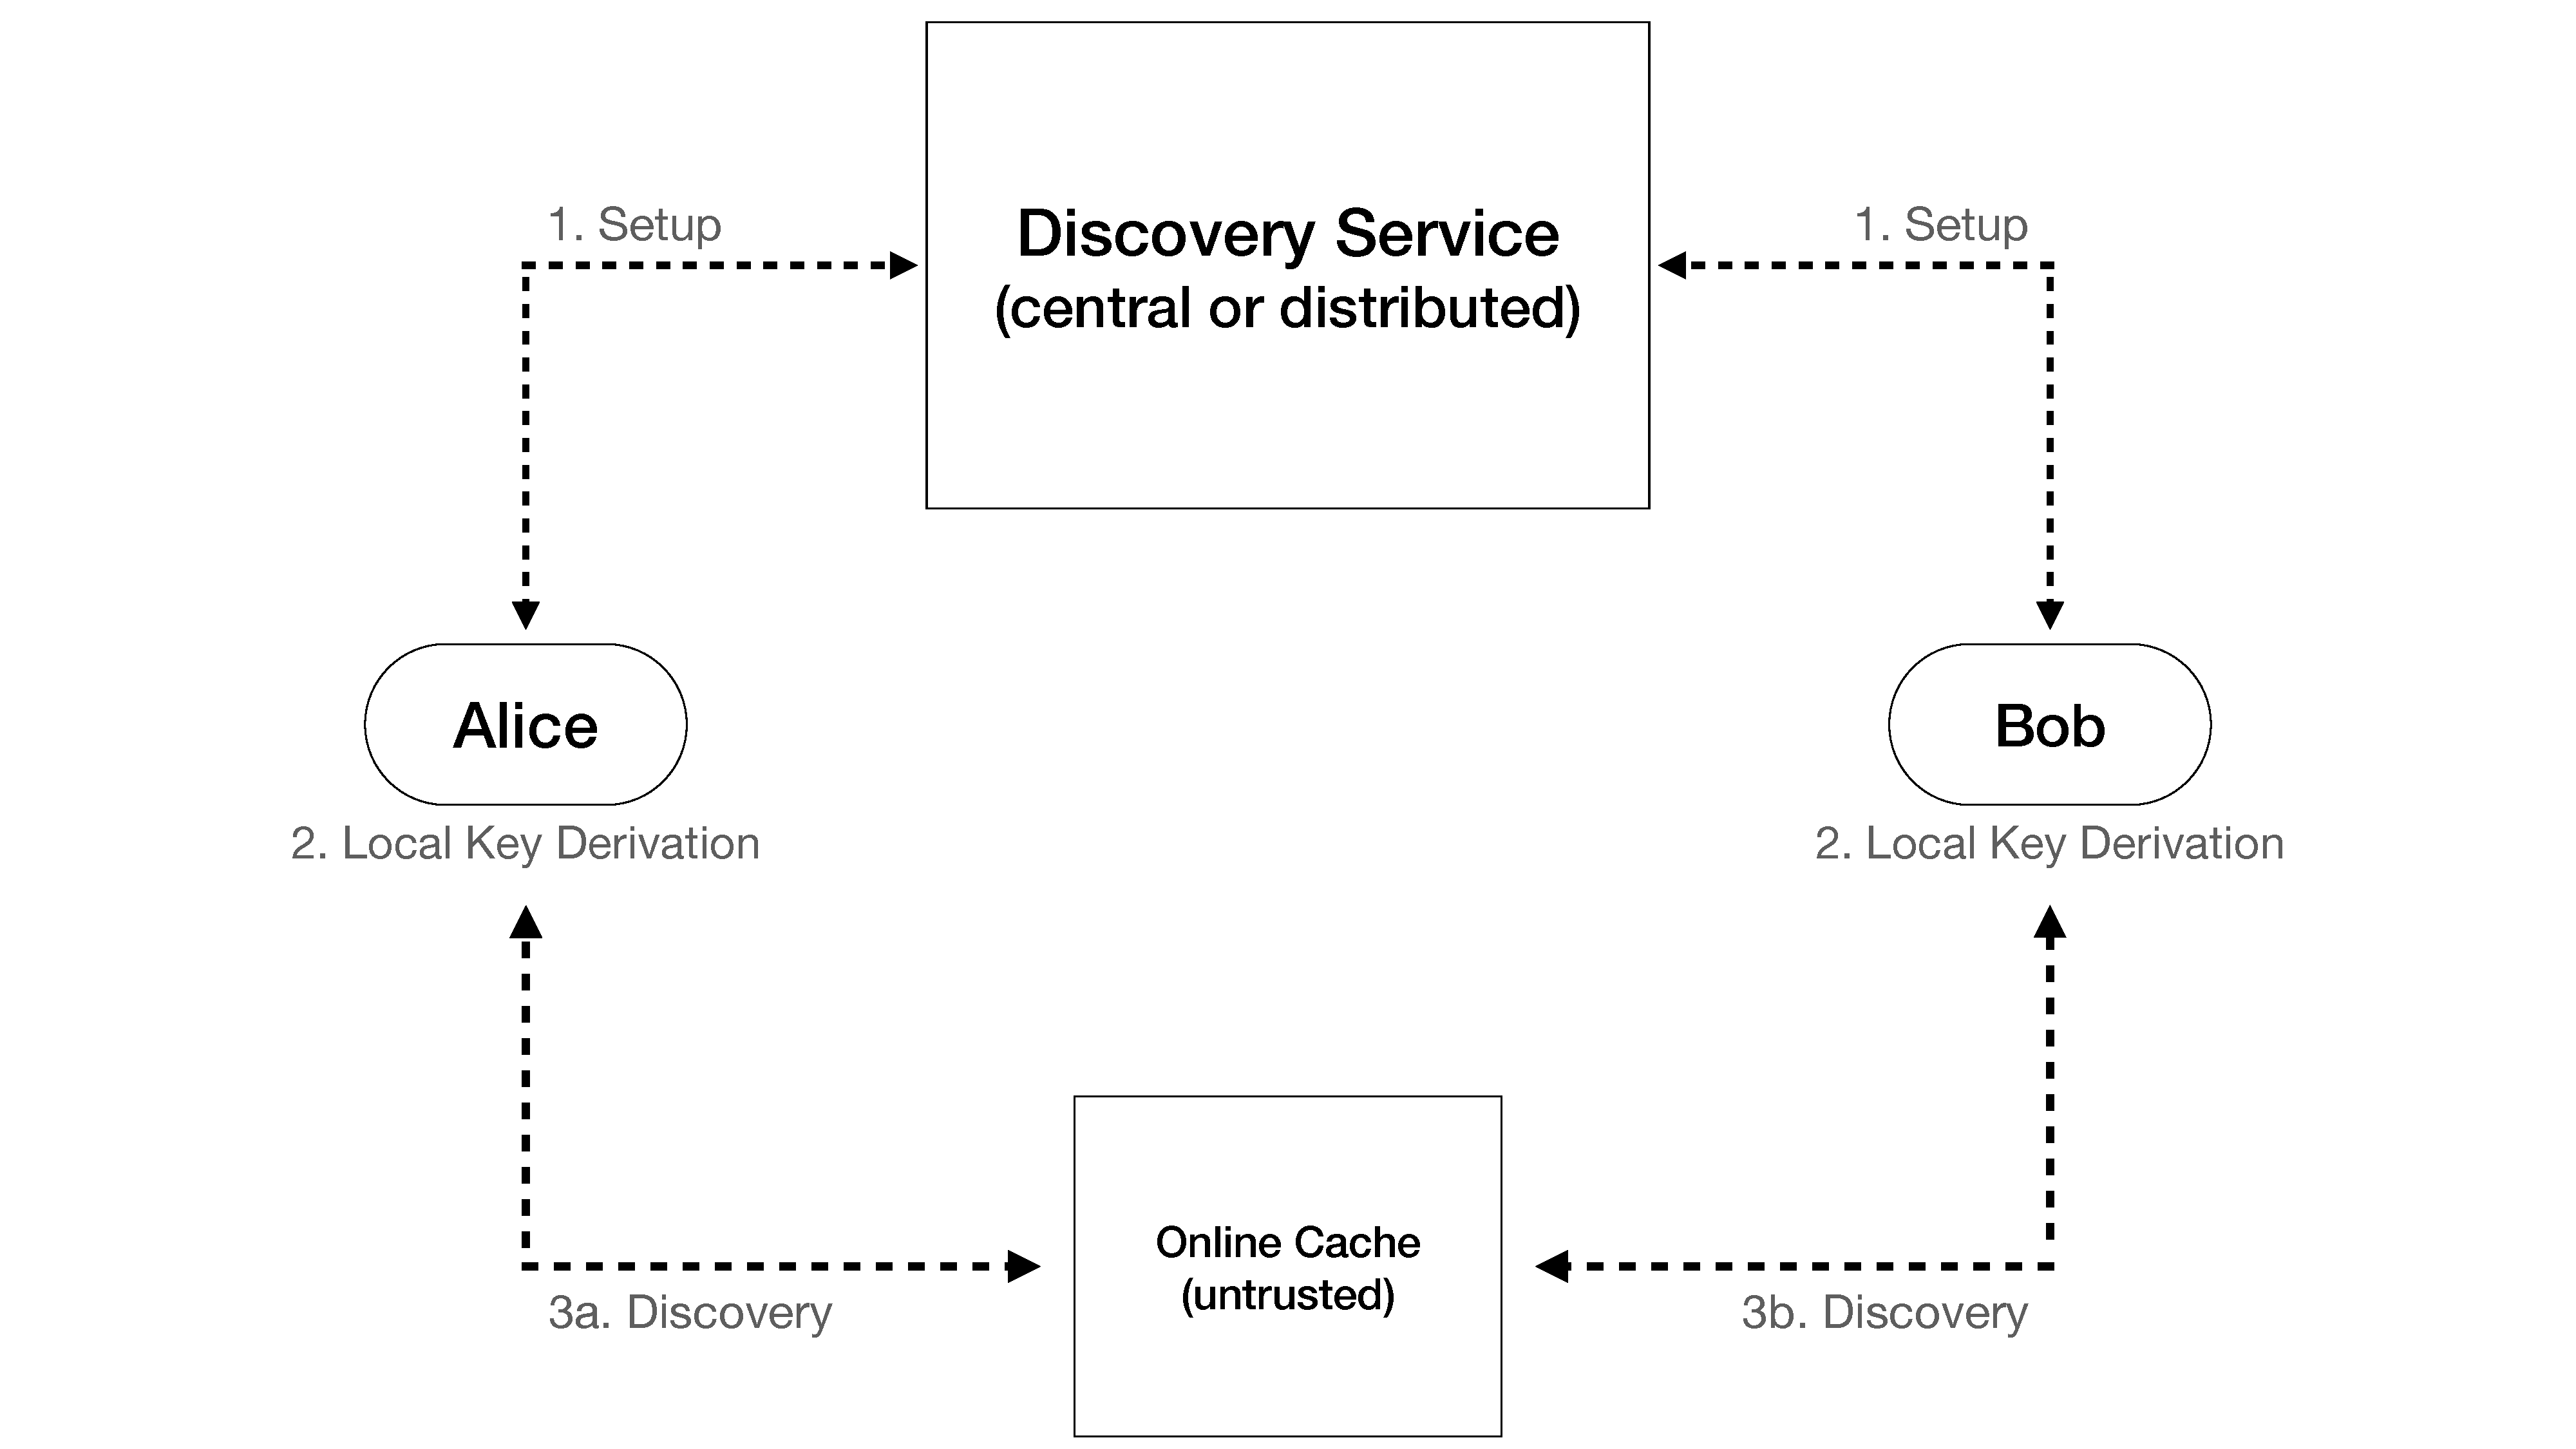
\includegraphics[width=\textwidth]{figures/system}
	  \caption{Contact discovery between a pair of users Alice and Bob, including setup. Numbers indicate the order of execution}
	  \label{fig:diagram}
	 \end{center}
 \end{figure}

	\subsection{Actors, assets and notation}
	
		\noindent We make a brief aside to clarify the actors and assets present in our scheme:		
		\begin{itemize}
			\item \textbf{Users:} each user $A$ holds an opaque account identifier $\acc_A$, an address $\addr_A$, a key pair $(\sk_A,\pk_A)$, a discovery identifier $\id_A$ and an address book $\contacts{A}$ (see \autoref{sec:probstatement}). We denote $\mathcal{ID}$ the set of all existing discovery identifiers.
			\item \textbf{Discovery Service:} the discovery service is a distributed entity. We denote the set of all servers as $\mathcal{S}$ and the $i$-th server as $S_i$. Each server holds a share $s_i$ of a master secret key $s$. Furthermore, each server holds a list of tuples $(\acc, \pk)$ for all registered users.
			\item \textbf{Online Cache:} the online cache may be operated by the discovery scheme or by a third party and is assumed to be untrusted. Its role is to manage key-value pairs.
			
			\end{itemize}
			
		\noindent Next we define the cryptographic setting for our scheme:
		\begin{itemize}
			\item $\Gzero, \Gone, \Gt$ are three cyclic groups of prime order $q$ such that there exists a pairing $e : \Gzero \times \Gone \rightarrow \Gt$.
			\item $H_0: \mathcal{ID}\rightarrow \Gzero$  and $H_1: \mathcal{ID} \rightarrow \Gone$ are two public hash functions modelled as random oracles.
			\item $F: \mathbb{Z}_q \times \mathcal{ID}^2  \rightarrow \Gt$ is a left/right constrained PRF defined as: \begin{equation}
				F(k, (\id_A, \id_B)) = F_k(\id_A, \id_B)= \Pair{H_0(\id_A)}{H_1(\id_B)}^k
			\end{equation}
			\item $\mathbf{KDF}$ is a public, deterministic key derivation function.
			\item $\Sign$ and $\Verif$ are the two algorithms of a probabilistic and secure signature scheme which makes use of the third-party provided user keys $(\sk_A,\pk_A)$ 
			\item The master secret key is set to an integer $s \in \mathbb{Z}_q$ chosen uniformly at random. We define two corresponding master public keys ${g_0}^s$ and ${g_1}^s$, for which there exists $i$ public shares denoted as ${g_0}^{s_i}$ and ${g_1}^{s_i}$ respectively.
			\item Let $n$ the number of servers ($n=|\mathcal{S}|$)) and $t$ a fixed threshold such that $1 \leq t \leq n$, we assume that the master secret key is shared according to a secure $t$-out-of-$n$ secret sharing scheme and that no single entity holds the master secret key.
		\end{itemize}

	\subsection{Key derivation}
	
		\paragraph{} We first introduce the essential key derivation step. In doing so, we provide the reader with the necessary material to understand the security constraints under which the initial setup phase operates.
		
		\paragraph{} For all users $B$ such that $\id_B \in \mathcal{C}_A$, user $A$ can compute shared key material with $B$ by evaluating $F_s(\id_A, \id_B)$ and $F_s(\id_B, \id_A)$. From the definition of left/right constrained PRFs, $A$ can do so with the constraining keys $\keyleft{\id_A}$ and $\keyright{\id_A}$:
		\begin{align}
			f_{AB} = F_s(\id_A, \id_B) &= \Pair{\keyleft{\id_A}}{H_1(\id_B)} \\
			f_{BA} = F_s(\id_B, \id_A) &= \Pair{H_0(\id_B)}{\keyright{\id_A}}
		\end{align} 
	
	\noindent Similarly, $B$ can evaluate $F$ at the same points using the constraining keys $\keyleft{\id_B}$ and $\keyright{\id_B}$:		
		\begin{align}
			f_{AB} = F_s(\id_A, \id_B) &= \Pair{H_0(\id_A)}{\keyright{\id_B}} \\
			f_{BA} = F_s(\id_B, \id_A) &= \Pair{\keyleft{\id_B}}{H_1(\id_A)} 
		\end{align}
	
\noindent Using this key material, $A$ and $B$ can establish a symmetric secret key using a standardised key derivation function:
	\begin{equation}
		k_{AB} = k_{BA} = \mathbf{KDF}\left(f_{AB} \xor f_{BA}\right)
	\end{equation}
	
	\paragraph{A note on security --} The constraining keys $\keyleft{\id_A}$ and $\keyright{\id_A}$ allow to compute every symmetric key that $A$ may establish with her contacts. As such, those \textbf{constraining keys must remain private} to $A$. The consequences of a leak range from impersonation to a total leak of $A$'s address book and are further detailed in \autoref{sec:security}.
	
	\subsection{Discovery}
	
		\paragraph{} Using their shared key material $(k_{AB}, f_{AB}, f_{BA})$, users $A$ and $B$ can determine secret memory locations on the online cache to leave an encrypted message for each other. Let $(\enc$, $\dec)$ be a secure symmetric encryption scheme and $H$ a hash function modelled as a random oracle, we define two cache operations $\mathbf{Write}$ and $\mathbf{Read}$:
		\begin{itemize}
			\item $\mathbf{Write}$: store the key-value pair $(H(f_{AB}), \enc_{k_{AB}}(\pk_A || \addr_A))$ on the online cache.
			\item $\mathbf{Read}$: retrieve the key-value pair $(H(f_{BA}), c_{BA})$. If $B$ has already run the discovery phase of our scheme then $c_{BA} = \enc_{k_{BA}}(\pk_B||\addr_B)$. Decrypt $c_{BA}$ using the key $k_{AB} = k_{BA}$.
		\end{itemize}
	
	\subsection{Setup}
	\label{sec:setup}
		
		\paragraph{}  The setup stage serves to provide user $A$ with the constraining keys $k_{\id_A,\mathrm{LEFT}}$ and $k_{\id_A,\mathrm{RIGHT}}$. Consequently, the setup is a security-critical task. As we have shown in \autoref{eq:constrkeys}, under our construction of $F$ the constraining keys can be expressed as:
		\begin{equation}
			k_{\id_A,\mathrm{LEFT}} = H_0(\id_A)^s \quad \mathrm{and} \quad k_{\id_A,\mathrm{RIGHT}} = H_1(\id_A)^s
		\end{equation}
		
		\noindent These constraining keys are equivalent to BLS signatures on $\id_A$ by at least $t$ out of $n$ servers of the discovery service. Notice that the service needs to produce signatures under both variants of the BLS scheme: one with signatures in $\Gzero$ and one with signatures in $\Gone$.
				
		\paragraph{} The setup protocol between user $A$ and a server $S_i$ is described as follows:
		\begin{enumerate}
			\item $A$ chooses a random blinding factor $\alpha \sample \mathbb{Z}_q$ and sends $\acc_A$, $\mathbf{sig}_A \leftarrow \Sign(\sk_A, \acc_A)$, $H_0(\id_A)^\alpha$, $H_1(\id_A)^\alpha$ to $S_i$.
			\item Upon reception of $A$'s request, $S_i$ retrieves the associated public key and checks that the signature $\mathbf{sig_A}$ is valid:
			\begin{equation}
				\Verif(\pk_A, \acc_A, \mathbf{sig}_A) = 1
			\end{equation}
		\item If the check succeeds, $S_i$ sends $(H_0(\id_A)^\alpha)^{s_i}$ and $(H_1(\id_A)^\alpha)^{s_i}$ to $A$
		\item Using $S_i$'s public key shares $({g_0}^{s_i}, {g_1}^{s_i})$, $A$ checks the following equalities:
		\begin{align}
			\Pair{(H_0(\id_A)^\alpha)^{s_i}}{g_0} &= \Pair{H_0(\id_A)^\alpha}{{g_0}^{s_i}} \\
			\Pair{g_1}{(H_1(\id_A)^\alpha)^{s_i}} &= \Pair{{g_1}^{s_i}}{H_1(\id_A)^\alpha}
		\end{align}
		\item If the checks succeed (in other words, if $A$ receives valid signatures from the service), $A$ removes the blinding factor $\alpha$ to obtain $H_0(\id_A)^{s_i}$ and $H_1(\id_A)^{s_i}$.
		\end{enumerate}
		
		
%\fbox{
%	\procedure{Setup}{%
%		\textbf{user } A  \< \<\textbf{server } S \\
%		\alpha \sample \mathbb{Z}_q \< \\
%		\mathbf{sig}_A = \Sign(\sk_A, \acc_A) \< \\
%		\<\sendmessageright{top={$\acc_A,\mathbf{sig}_A, H_0(\id_A)^\alpha, H_1(\id_A)^\alpha$} } \\
%		\<\< \text{If } \Verif(\pk_A, \acc_A, \mathbf{sig}_A) = 0 \\
%		\<\< \qquad\textbf{Abort}\\
%		\<\< \text{Else}\\
%		\< \sendmessageleft{top={$(H_0(\id_A)^\alpha)^s, (H_1(\id_A)^\alpha)^s$}} 
% }
% }
	
	\paragraph{} $A$ repeats the above procedure with at least $t$ servers, using a new blinding factor for each server. Using the obtained signature shares, $A$ can recover the full signatures $H_0(\id_A)^s$ and $H_1(\id_A)^s$.
	
	


\section{Privacy}
\label{sec:security}


\paragraph{} We will now evaluate the privacy guarantees of our scheme when there are strictly less than $t$ malicious servers. At first, we work under the assumption that discovery identifiers are correctly linked to the users who own them. We then discuss ways in which this assumption can be upheld in practice.





	\subsection{Threat model}
	\paragraph{} An adversary $\Tadv$ wishing to break our scheme's privacy property aims to gain information about the contents of any user's address book. This goal is equivalent to determining whether $\id_B \in \contacts{A}$ for any user $A$ and any identifier $\id_B$ that is not owned by $\Tadv$. $\Tadv$ is characterised as:
	\begin{itemize}
		\item having access to all public information.
		\item having access to the present and past states of the online cache.
		\item may eavesdrop on any communication between the users, servers and online cache.
		\item may spawn any number of users for which $\Tadv$ owns the discovery identifier.
		\item may control up to $t-1$ servers in the discovery service.
	\end{itemize}
	
	
	\paragraph{} To guide our analysis, we provide an attack tree\footnote{as defined by Schneier \cite{attacktree}} against the privacy property of our scheme in \autoref{fig:attacktree}. The root node represents the attacker's goal and each child node represents an option to solve the problem indicated in the parent node. Consequently leaf nodes represent the attacker's entry points. We will therefore consider each leaf and show that our scheme is protected against these attacks.
	
	
		\begin{figure}[H]
			\begin{center}
				\begin{center}
	

\begin{forest}
for tree={
  draw,
  minimum height=1cm,
  anchor=north,
  align=center,
  child anchor=north
},
[{Learn whether $\id_B \in \contacts{A}$}, align=center, name=SS
  [{Distinguish key-value pair\\ $(H(f_{AB}), \enc_{k_{AB}}(\pk_A || \addr_A))$\\ on online cache from random}, name=PDC
    [{Distinguish $f_{AB}$ from random}
    	[Break security\\ property of $F$\\ (definition \autoref{def:lrPRFsec})]
    	[Obtain $s$]
    	[{Obtain $A$'s\\ constraining keys}
    		[Forge BLS signatures]
    		[Impersonate $A$]
    	]
    ]
    [Decrypt $\enc_{k_{AB}}(\pk_A || \addr_A))$
    	[Compute $k_{AB}$]
    ]
  ]
]
\end{forest}

\end{center}
				\caption{Attack tree against our discovery scheme. Branches represent ``OR'' statements}
				\label{fig:attacktree}
			\end{center}
		\end{figure}

	
	
%		\paragraph{} Our scheme reduces the contact discovery problem to the evaluation of a left/right constrained PRF at two specific points, namely $(\id_A, \id_B)$ and $(\id_B, \id_A)$. Indeed an adversary trying to uncover a link between users $A$ and $B$ without computing their shared key material will face two obvious hurdles. Firstly, such an adversary will be unable to find $A$ and $B$'s meeting point on the online cache other than by exhaustively iterating through all possible location. Furthermore, since $H$ is modelled as a random oracle, this adversary will be unable to distinguish this location from any other. The second issue is that the value stored in that location is encrypted under $k_{AB}$. Therefore, to uncover the link between $A$ and $B$, an adversary will need to evaluate the left/right constrained PRF at the correct points.
		
		
%		\paragraph{} We provide a formal definition of secure left/right constrained PRFs by using an attack game. We will then show that the construction used in our scheme meets the security definition.
		
		
		
		\begin{theorem}
			The PRF $F$ defined as $F(k, (x,y)) = \Pair{H_0(x)}{H_1(y)}^k$ is a secure constrained PRF with respect to its constraining keys assuming the decisional bilinear Diffie-Hellman assumption holds for $e$ and the functions $H_0$ and $H_1$ are modelled as random oracles.
		\end{theorem}
		


	\subsection{Consequences of a breach}
	
	\subsection{Authentication: an open problem}


\section{Theoretical performance evaluation}
\label{sec:performance}


\section{Applications}
\label{sec:applications}

	\subsection{End-to-end encrypted messaging}
	
	\subsection{Mobile-first cryptocurrencies}

\chapter{Proof-of-Concept Implementation}
\label{chap:implementation}


\paragraph{} We now describe a proof-of-concept implementation of the contact discovery service written in Go. At the time of writing, this proof-of-concept performs setup locally by emulating the behaviour of the distributed discovery service. Key derivation is performed locally as expected. Finally, a meeting point is established via the InterPlanetary FileSystem (IPFS)\footnote{\url{https://ipfs.io}}. It is important to highlight that the IPFS is a content-addressed system: rather than storing key-value pairs, the IPFS derives a key as a function of the value. This behaviour does not match our requirements for the online cache, but allows us to establish a meeting point and perform contact discovery nonetheless.




\section{Local server emulation}

	\paragraph{} To emulate the behaviour of our distributed discovery service, we need to create $n$ \texttt{server} objects, perform a $t$-out-of-$n$ threshold distributed key generation (DKG) algorithm and implement BLS signatures in both source groups of an asymmetric pairing. We make use of the \kyber \;library\footnote{\url{https://github.com/dedis/kyber}} to provide most of the cryptographic backend. This library performs pairing operations on the BN256 elliptic curve.
	
	\paragraph{Server representation --} We are performing a local emulation and therefore choose to abstract from network properties such as a server's address. We however include an \texttt{ID} field that represents any such identifying information. Consequently, our model for a server is as simple as possible: it includes an identifier, a secret key share for the BLS signature scheme in $\Gzero$ and a secret key share for the BLS signature scheme in $\Gone$ (see \autoref{fig:server_def}).
	
	\begin{figure}[H]
		\begin{center}
			\begin{lstlisting}
	type multiServer struct {
		ID  int
		sk1 *share.PriShare
		sk2 *share.PriShare
	}
			\end{lstlisting}
			\caption{Implementation: definition of a server}
			\label{fig:server_def}
		\end{center}
  	\end{figure}
  	
  	\paragraph{Distributed Key Generation --} Rather than performing a distributed key generation algorithm, we assume the existence of a trusted dealer and perform key distribution by sharing a random secret (see \autoref{fig:key_distrib}). As DKG algorithms are not the primary focus of our report, this assumption allows for a simple setup for our proof-of-concept implementation. We perform secret sharing using \kyber's \texttt{share} package. Finally, for testing purposes, we have hard-coded a master secret key, thus allowing experiments to be reproducible. 
  	
  	\begin{figure}[H]
		\begin{center}
		\begin{lstlisting}
func setupThresholdServers(suite pairing.Suite, secret kyber.Scalar, n, t int) ([]*multiServer, *share.PubPoly, *share.PubPoly) {
	serverList := make([]*multiServer, n)
	if secret == nil {
		secret = suite.GT().Scalar().Pick(random.New())
	}

	priPoly1 := share.NewPriPoly(suite.G2(), t, secret, random.New())
	pubPoly1 := priPoly1.Commit(suite.G2().Point().Base())
	serverPrivateKeys1 := priPoly1.Shares(n)

	priPoly2 := share.NewPriPoly(suite.G1(), t, secret, random.New())
	pubPoly2 := priPoly2.Commit(suite.G1().Point().Base())
	serverPrivateKeys2 := priPoly2.Shares(n)

	for i := 0; i < n; i++ {
		serverList[i] = newMultiServer(i, serverPrivateKeys1[i], serverPrivateKeys2[i])
	}

	return serverList, pubPoly1, pubPoly2
}
		\end{lstlisting}
	\caption{Implementation: Key distribution using a trusted dealer}
		\label{fig:key_distrib}
		\end{center}
	\end{figure}


  	\paragraph{Blind $(t,n)$-threshold BLS --} To complete our server emulation, we implement blind $(t,n)$-threshold BLS signature schemes in both variants (with signatures in $\Gzero$ and in $\Gone$). The \kyber\;library only allows signatures in $\Gzero$ and takes messages as inputs to its signing algorithm. As such, we are unable to manipulate hashes of those messages; more specifically we are unable to blind and unblind our messages. We therefore implement a slight variant of the existing library to allow for blinding and introduce the necessary functions to performs BLS signatures on elements of $\Gone$  (see packages \hyperref[app:morebls]{\texttt{morebls}} , \hyperref[app:moretbls]{\texttt{moretbls}}, \hyperref[app:blindbls]{\texttt{blindbls}}, \hyperref[app:blindtbls]{\texttt{blindtbls}} in \autoref{app:code}). We do not however implement a secure hash-to-$\Gone$ method as should be the case in a production-grade service.
  	
  	\paragraph{} Using the above setup, clients are able to send their blinded discovery identifiers to any of the $n$ emulated servers. The servers respond by providing a BLS signature using their private key shares (see lines 68--74 of \autoref{lst:server} in \autoref{app:code}). We do not however implement many of the identity checks that are required to provide a secure setup.
  	
  	
  	  	
\section{User-facing client application}

	\paragraph{Users --} We consider that each user runs an instance of our client application presented here. Users are therefore prompted to enter their discovery identifier upon first launch. This identifier is then hashed to both source groups to produce public keys \texttt{pk1} and \texttt{pk2}. Once the user completes the setup process, she will receive her left and right constraining keys. We call these the user's secret keys \texttt{sk1} ans \texttt{sk2} to emphasise the fact that both keys must remain private at all times. Users are therefore represented using the data structure shown in \autoref{fig:user_def}.
	
	\begin{figure}[H]
	\begin{center}
		\begin{lstlisting}
	type user struct {
		name               string
		phoneNumber        string
		pk1, pk2, sk1, sk2 kyber.Point
	}
		\end{lstlisting}
	\caption{Implementation: definition of a user}
	\label{fig:user_def}
	\end{center}
\end{figure}


	\paragraph{User setup --} Upon launching the application, users receive a list of available servers and the setup threshold $t$. The client application performs the setup process by interacting with $t$ servers of its choice. Each interaction consists of blinding the user's public keys, verifying the received signature and unblinding it to store shares of the constraining keys. When enough shares are gathered, the client application runs the $\Combine$ algorithms from each of the two threshold BLS schemes (see lines 108--173 of \autoref{lst:user} in \autoref{app:code}).



	\paragraph{Key derivation --} Using a user's constraining keys and a contact's discovery identifier, the client application can evaluate the left/right constrained PRF by performing two pairing operations (see \autoref{fig:key_deriv}).
	
	\begin{figure}[H]
	\begin{center}
		\begin{lstlisting}
	// Derive shared keys between users A and B:
	// shared12 = e(H1(idA)**s, H2(idB)) = e(H1(idA), H2(idB))**s
	// shared21 = e(H1(idB), H2(idA)**s) = e(H1(idB), H2(idA))**s
	func deriveSharedKeys(alice *user, contactNumber string) (kyber.Point, kyber.Point) {
		bobPk1, bobPk2 := derivePublicKeys(contactNumber)
		shared12 := suite.Pair(alice.sk1, bobPk2)
		shared21 := suite.Pair(bobPk1, alice.sk2)
	
		return shared12, shared21
	}
		\end{lstlisting}
	\caption{Implementation: local key derivation}
	\label{fig:key_deriv}
	\end{center}
\end{figure}



\section{Online meeting point via IPFS}

	\paragraph{} The final step required to successfully perform contact discovery is to establish an online meeting point. As mentioned above, the IPFS is not originally a key-value store. We therefore develop another approach to the discovery phase which slightly differs from that presented in \autoref{chap:system}.
	
	\paragraph{} The IPFS is a content-addressed storage system in which the location of an object is its hash. Therefore, we modify the discovery phase such that both parties $A$ and $B$, can compute two pieces of unique, secret content $c_{AB}$ and $c_{BA}$. These are in fact ciphertexts under the symmetric key $k_{AB} = k_{BA}$ for standardised plaintexts such that both users can locally compute them. To check whether $B$ is registered to an application, $A$ can check whether $c_{BA}$ is available on the IPFS. Similarly, $B$ can check for the presence of $c_{AB}$. Notice however that we cannot encrypt information that is not shared between $A$ and $B$. Indeed, doing so would mean that one of the two parties is unable to compute the hash --- and therefore the IPFS address --- of one of the ciphertexts. As a result, this simplified method does not allow to transfer information during the contact discovery phase. Users may only receive and send binary information by uploading or withholding their ciphertexts.
	
	\paragraph{} The IPFS provides simple command-line tools to upload and access files from its peer-to-peer network. Using these tools, $A$ uploads $c_{AB}$ and tries to retrieve $c_{BA}$. If the file is available, $A$ knows $B$ is a registered user. Otherwise, the IPFS instruction will time out and $A$ will learn that $B$ is not registered. This process implies that $c_{AB}$ and $c_{BA}$ must remain available on the IPFS network regardless of either users' connection status. Fortunately, the IPFS implements a ``pinning'' mechanism to ensure that files are stored by more than one node and made available at all times.


\section{Observations and further steps}


\paragraph{} This simple proof-of-concept application demonstrates the feasibility of a contact discovery scheme built according to our architecture. As expected, our implementation allows users to obtain constraining keys by gathering and combining blind BLS signatures on their discovery identifiers. The key derivation step provides consistent shared key material between two users that know each other's discovery identifier. Finally, we have shown that the shared key material can be used to establish contact online.


\paragraph{} The next step in further demonstrating the feasibility of our architecture is benchmarking. To do so, we wish to develop a server-side application that runs online and integrate our discovery scheme in a custom-modified mobile application such as Signal or Celo's mobile clients (similarly to the experiments ran by Kales \textit{et al.} \cite{Kales19}). This test-bed will allow us to measure the scheme's cost in terms of computations and communication time as well as battery requirements in real-world conditions.
































\chapter{Conclusion}
\label{chap:conclusion}

\addcontentsline{toc}{chapter}{Appendices:}

\appendix

\chapter{Bilinear variants of the CDH and DDH problems}
\label{ap:coCDH}

\section{The co-computational Diffie-Hellman (co-CDH) Problem and Assumption}

	\paragraph{} The co-Computational Diffie-Hellman (co-CDH) assumption is a variant of the Computational Diffie-Hellman assumption that applies for asymmetric pairings. Let us recall the definition for the co-Computational Diffie-Hellman assumption given in \cite{BonehShoup}, using a multiplicative notation for the group operation as in the source text.. 
	
	\begin{secgame}[co-CDH \cite{BonehShoup}]
	\label{game:coCDH}
		Let $\Gzero, \Gone, \Gt$ be three cyclic groups of  prime order $q$ such that there exists a pairing $e : \Gzero \times \Gone \rightarrow \Gt$. For a given adversary \adv, the attack game runs as follows:
			\begin{itemize}
				\item The challenger picks at random $\alpha,\beta \sample \mathbb{Z}_q$ and computes
				 $$
				 	u_0 \leftarrow {g_0}^\alpha, \quad\quad u_1 \leftarrow {g_1}^\alpha, \quad v_0 \leftarrow {g_0}^\beta, \quad z_0 \leftarrow {g_0}^{\alpha\beta}
				 $$
				\item The adversary $\adv$ receives the tuple $(u_0, u_1, v_0)$ and outputs $\hat z_0 \in \Gzero$
						
			\end{itemize} 
	\end{secgame}
	
	\noindent We define the advantage of $\adv$ in solving the co-CDH problem for $e$ as:
	\begin{equation}
		\mathrm{coCDHadv}[\adv, e] := \mathrm{Pr}(\hat z_0 = z_0)
	\end{equation}
	
	\noindent Notice that for symmetric pairings, $\Gzero = \Gone$ therefore $g_0 = g_1 $, $u_0 = u_1$ and attack game \autoref{game:coCDH} is identical to the Computational Diffie-Hellman attack game.
	
	\begin{definition}[co-CDH Assumption \cite{BonehShoup}]
		We say that the co-CDH assumption holds for the pairing $e$ if for all efficient adversaries $\adv$ the quantity $\mathrm{coCDHadv}[\adv, e]$ is negligible.
	\end{definition}
	
\section{The decision bilinear Diffie-Hellman (DBDH) Problem and Assumption}

\paragraph{} The decisional variant is relatively straight-forward having already defined the co-CDH assumption. The attack setting is closely related, however the adversary is expected to distinguish an element from random (rather than required to computed it). Once again, the definition is adapted from \cite{BonehShoup} and uses a multiplicative notation for group operations.

\begin{secgame}[Decision bilinear Diffie-Hellman \cite{BonehShoup}]\label{att:DBDH}
	Let $e : \Gzero \times \Gone \rightarrow \Gt$ be a pairing where $\Gzero,\Gone,\Gt$ are cyclic groups of prime order $q$ with generators $g_0 \in \Gzero$ and $g_1 \in \Gone$. For a given adversary $\adv$, we define the following experiment:
	
	\begin{itemize}
		\item The challenger picks at random $ \alpha, \beta, \gamma, \delta \sample \mathbb{Z}_q $,
			computes $$ u_0 \leftarrow {g_0}^\alpha, \quad u_1 \leftarrow {g_1}^\alpha, \quad v_0 \leftarrow {g_0}^\beta, \quad w_1 \leftarrow {g_1}^\gamma, \quad z^{(0)} \leftarrow {g_0}^{\alpha\beta\gamma}, \quad z^{(1)} \leftarrow {g_0}^\delta $$
			and flips a bit $b\sample\{0,1\}$. Using the result of the bit flip, the challenger sends $(u_0, u_1, v_0, w_1, z^{(b)})$ to $\adv$.
		\item $\adv$ receives $(u_0, u_1, v_0, w_1, z^{(b)})$ and outputs a bit $\hat b \in \{0,1\}$
	\end{itemize}
\end{secgame}

\noindent We define the advantage of $\adv$ in solving the DBDH problem for $e$ as:

\begin{equation}
	\mathrm{DBDHavd}[\adv, e] := \abs{\frac{1}{2} - \mathrm{Pr}(\hat b = b)}
\end{equation}

\begin{definition}[Decision BDH assumption \cite{BonehShoup}]
	We say that the decision bilinear Diffie- Hellman assumption holds for the pairing $e$ if for all efficient adversaries $\adv$ the quantity $\mathrm{DBDHavd}[\adv, e]$ is negligible.
\end{definition}



\chapter{Calculations: performance evaluation}



% TODO jupyter notebook














\chapter{Code}



% BIBLIOGRAPHY
\newpage
\addcontentsline{toc}{chapter}{Bibliography}
\bibliographystyle{splncs03}
\bibliography{references}

\end{document}
